\documentclass{article}
\usepackage{fullpage}
%%% Работа с русским языком
\usepackage[T2A]{fontenc}
\usepackage[utf8]{inputenc}
\usepackage[english,russian]{babel}   %% загружает пакет многоязыковой вёрстки
\usepackage{indentfirst}
\frenchspacing
\usepackage{titlesec} % package to customize chapters, sections and subsections style
%--------------------------------------
\titleformat{\section}{\large\bfseries\centering}{\thesection}{1em}{}
%Hyphenation rules
%--------------------------------------
\usepackage{hyphenat}
\hyphenation{мате-мати-ка восста-навливать}
%--------------------------------------
\usepackage{amsmath}
\usepackage{amssymb}
\usepackage[bb=pazo,frak=pxtx,frakscaled=1.3]{mathalfa}
\usepackage{upgreek}
\usepackage{graphicx}
\title{Контрольная работа № 1 по курсу «Дискретная математика»}
\author{Ригованов Филипп Юрьевич, студент группы КТбз1-1}
\begin{document}
\date{}
\maketitle
\section*{Раздел № 1. Основные определения. Способы задания множеств.}
24. Задать множество $D = \{2, 4, 6, 8, 10, 12, 14, 16, 18\}$ высказывательным способом.

Ответ: $D = \{x \;| \; (\exists y)( y \in \mathbb{N} \;\&\; y < 10 \;\&\; x = 2y)\}$.
\section*{Раздел № 2. Операции над множествами.}
24. Для произвольных множеств $A , B , C  \in  \mathfrak{R}(E)$ доказать или опровергнуть тождество \\ $A \setminus (A \setminus B) = A \cap B$ методом взаимного включения множеств.

\begin{center}Решение:\end{center}

1) Докажем необходимость $A \setminus (A \setminus B) \subseteq A \cap B$:

$$x \in A \setminus (A \setminus B) \rightarrow x \in A \;\;\&\;\; x \notin A \setminus B \rightarrow x \in A \;\;\&\;\; (x \notin A \;\vee\; x \in B) \rightarrow x \in A \;\;\&\;\; x \notin A \;\vee\; x \in A \;\;\&\;\; x \in B \rightarrow$$
$$ \rightarrow x \in \varnothing \;\vee\; x \in A\cap B \rightarrow x \in A\cap B.$$

2) Докажем достаточность $A \setminus (A \setminus B) \supseteq A \cap B$:

$$x \in A\cap B \rightarrow x \in A \;\;\&\;\; x \in B \rightarrow x \in A \;\;\&\;\; x \in B \;\vee\; x \in \varnothing \rightarrow x \in A \;\;\&\;\; x \in B \;\vee\; x \in A \;\;\&\;\; x \notin A \rightarrow$$

$$\rightarrow x \in A \;\;\&\;\; (x \in B \;\vee\; x \notin A) \rightarrow x \in A \;\;\&\;\; x \notin A \setminus B \rightarrow x \in A \setminus (A \setminus B).$$

3) Доказав неоходимость и достаточность мы доказали тождество $A \setminus (A \setminus B) = A \cap B$.

\section*{Раздел № 3. Декартово произведение множеств.}
24. Для какого множества справедливо: $A = A^{-1}$ , если $A \subseteq X \times  Y$.

\begin{center}Решение:\end{center}

Очевидно условие задачи справедливо для симметричных бинарных отношений, ведь вместе с любым из своих элементов, оно должно содержать и обратный ему. Покажем это: воспользовавшись условием $A = A^{-1}$ можем записать $A=A\cup A=A\cup A^{-1}$, а множество $A\cup A^{-1}$ - всегда симметрично.

\section*{Раздел № 4. Соответствия и отношения.}
24. Для соответствий $\Gamma = \langle X, Y, F\rangle$ и $\Delta = \langle W, Z, P\rangle$, где $X = \{1, 2, 3,
4\}; Y = \{a, b, c, d\};\\ F = \{\langle 1, a\rangle; \langle 1, c\rangle; \langle 1, d\rangle; \langle 2, b\rangle; \langle 2, c\rangle; \langle 3, a\rangle; \langle 3, d\rangle;
\langle 4, b\rangle; \langle 4, c\rangle\}; W = \{a, c, d, e\}; Z = \{I, II, IV, V, VI\};\\ P = \{\langle a, I\rangle; \langle a, IV\rangle;
\langle a, V\rangle; \langle c, II\rangle; \langle c, IV\rangle; \langle d, II\rangle; \langle d, V\rangle; \langle d, VI\rangle; \langle e, I\rangle\}$ и произвольных множеств\\ $A = \{1, 2, 4\}$ и $B = \{a, c, d\}$ найти $\Delta^{-1} \circ \Gamma^{-1}$.

\begin{center}Решение:\end{center}

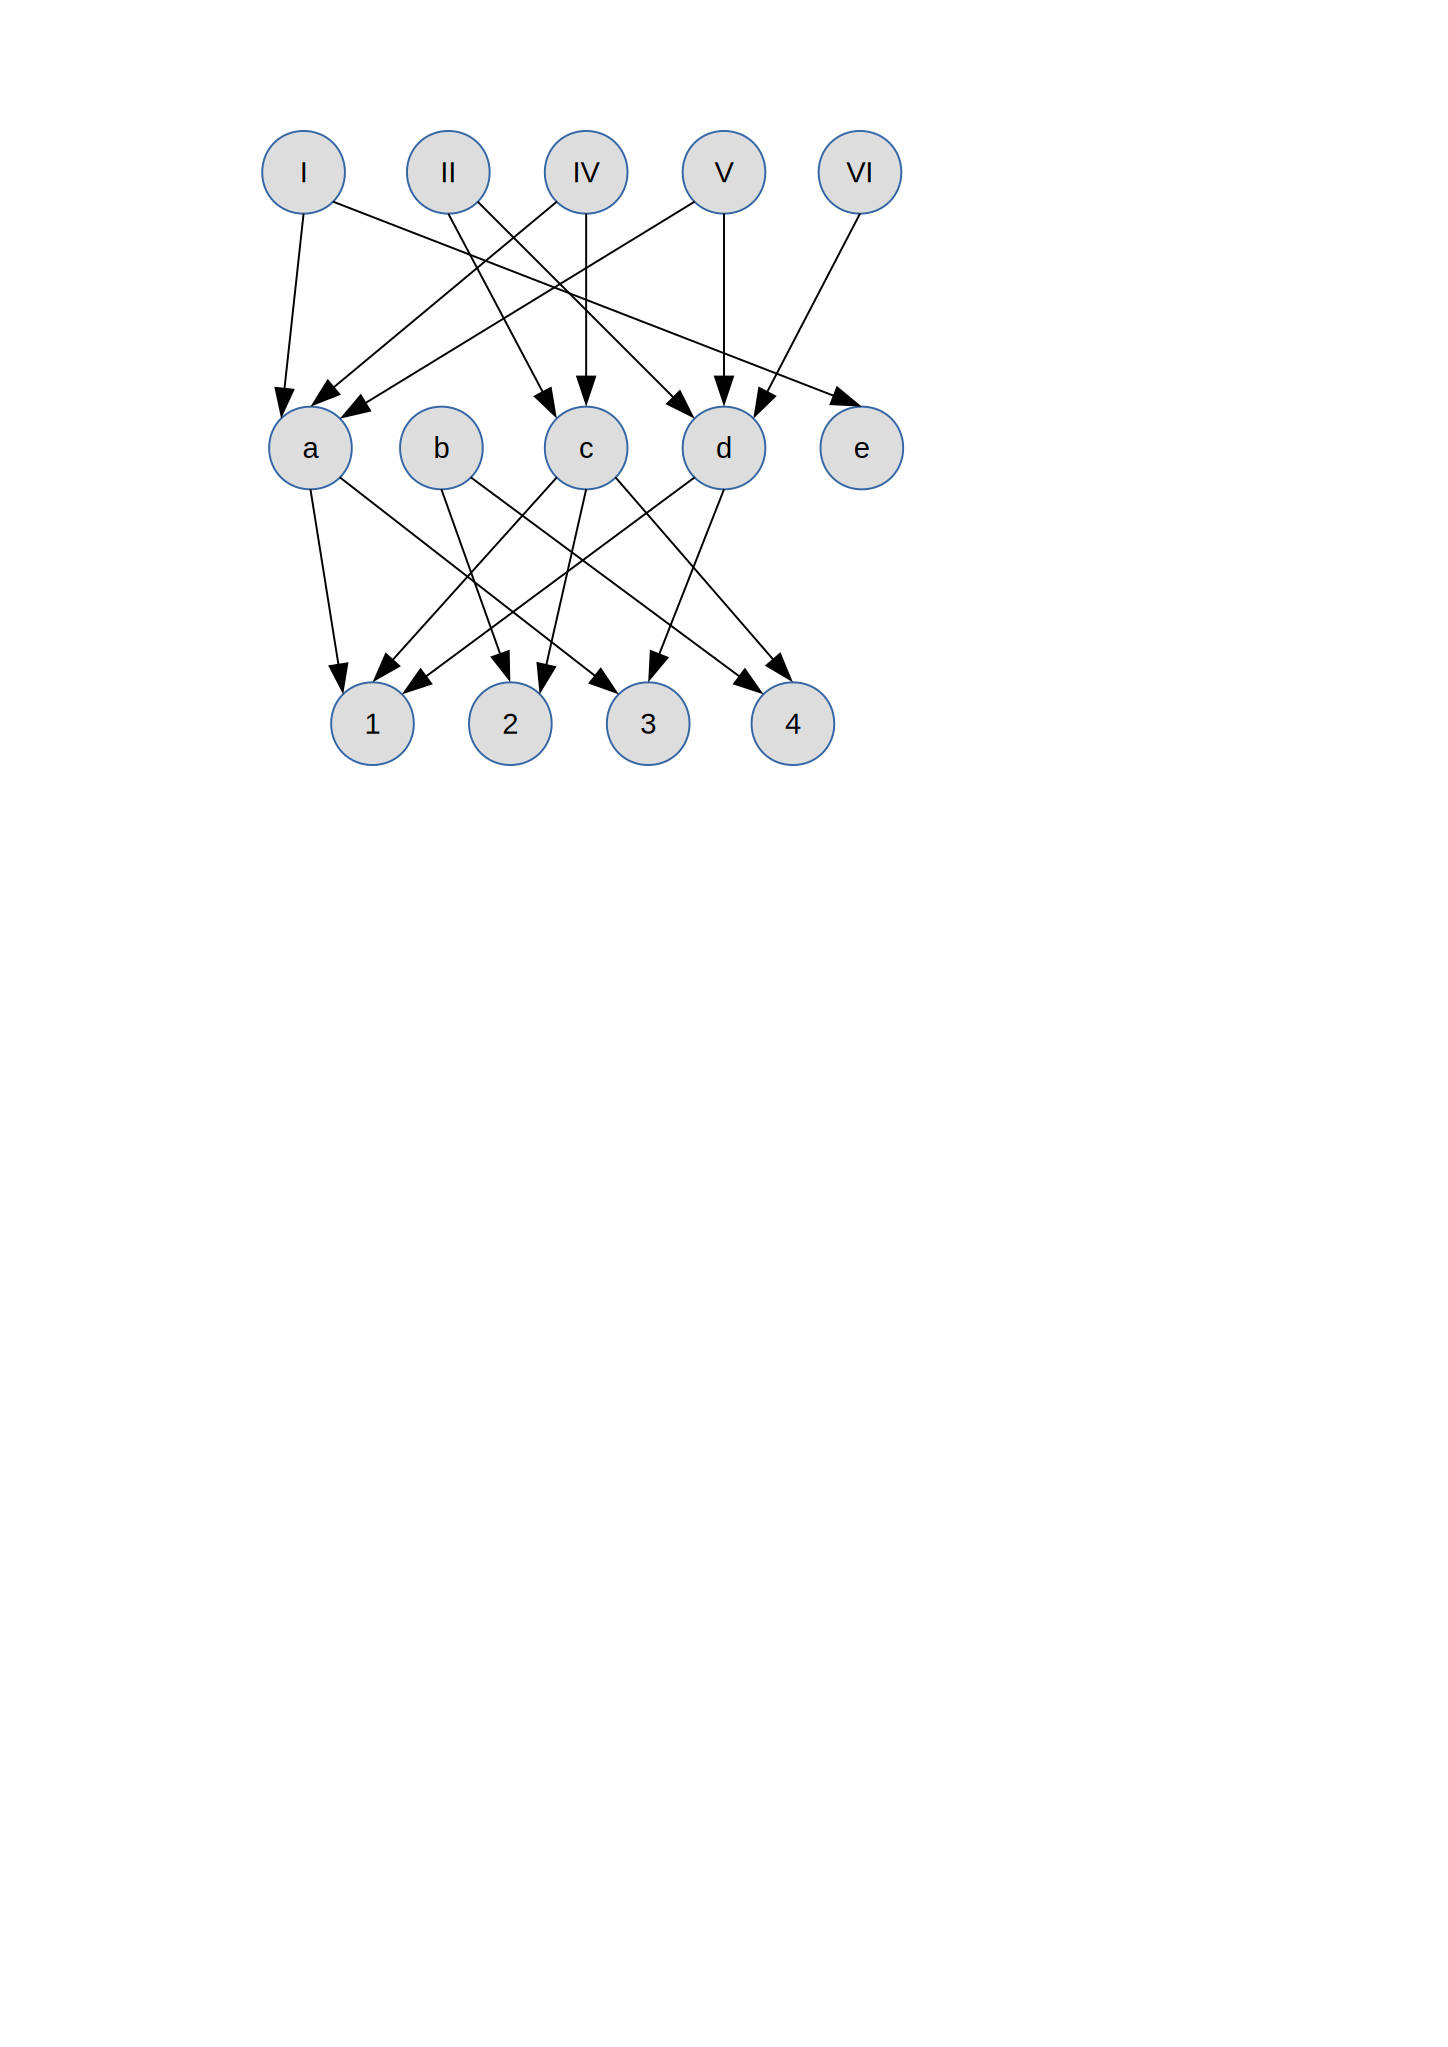
\includegraphics[width=200pt,natwidth=337,natheight=334]{/Users/phil/my/tex/src/4_1.png}
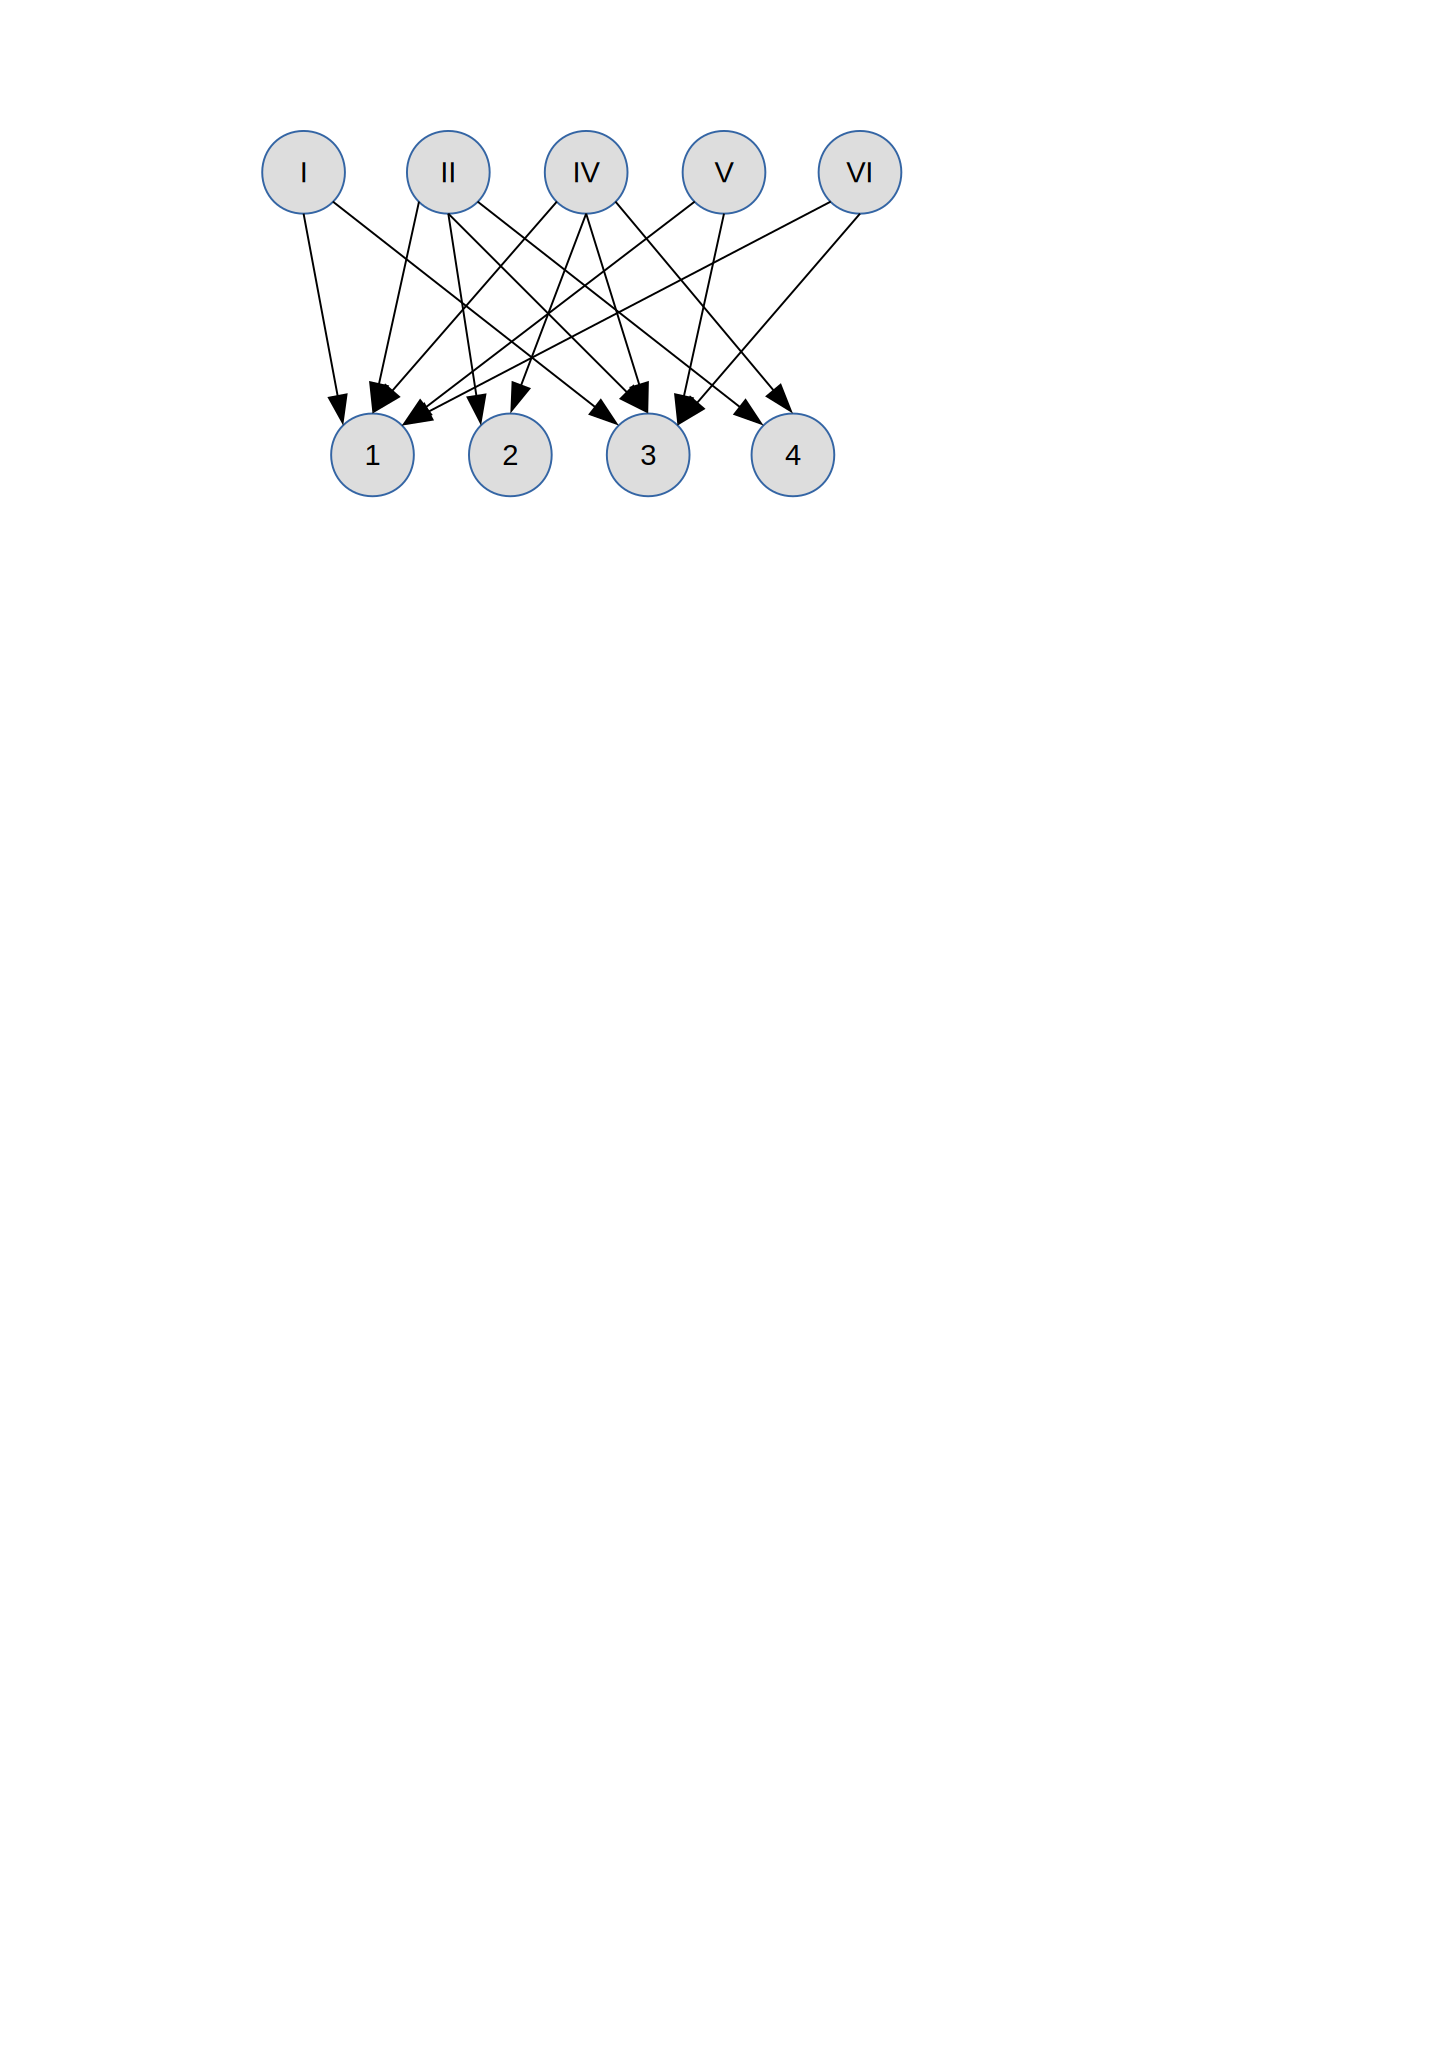
\includegraphics[width=200pt,natwidth=336,natheight=196]{/Users/phil/my/tex/src/4_2.png}

$\Delta^{-1} \circ \Gamma^{-1}=\langle U, V, E\rangle$, где
$U=\{I, II, IV, V, VI\}$, $V=\{1, 2, 3, 4\}$, $E=\{\langle I,1\rangle;
\langle I,3\rangle; \langle II,1\rangle; \langle II,2\rangle; \langle II,3\rangle;\\ \langle II,4\rangle; \langle IV,1\rangle; \langle IV,2\rangle; \langle IV,3\rangle; \langle IV,4\rangle;\langle V,1\rangle; \langle V,3\rangle;\langle VI,1\rangle; \langle VI,3\rangle;\}$

Так как множество $U=\{I, II, IV, V, VI\}$ не имеет общих элементов с множествами $A = \{1, 2, 4\}$ и $B = \{a, c, d\}$, то $\Delta^{-1} \circ \Gamma^{-1} (A)= \Delta^{-1} \circ \Gamma^{-1} (B) = \varnothing$.

\section*{Раздел № 5. Нечёткие высказывания и множества.}
24. Для нечётких соответствий $\widetilde{\Gamma} = \langle X, Y, \widetilde{F}\rangle$ и $\widetilde{\Delta} = \langle Y, Z, \widetilde{P}\rangle$, где $X = \{x_1, x_2, x_3, x_4\}, Y = \{y_1, y_2, y_3, y_4, y_5\},\\ \widetilde{F} = \{\langle 0.7, \langle x_1, y_2\rangle\rangle; \langle 0.9, \langle x_1, y_5\rangle\rangle;
\langle 0.1, \langle x_5, y_1\rangle\rangle; \langle 0.3, \langle x_2, y_2\rangle\rangle; \langle 0.6, \langle x_2, y_3\rangle\rangle; \langle 1, \langle x_3, y_4\rangle\rangle; \langle 0.8, \langle x_4, y_2\rangle\rangle;
\langle 0.4, \langle x_4, y_3\rangle\rangle\},\\ Y = \{y_1, y_2, y_3, y_4\}, Z = \{z_1, z_2, z_3\}, \widetilde{P} = \{\langle 0.6, \langle y_1, z_1\rangle\rangle; \langle 0.3, \langle y_1, z_2\rangle\rangle; \langle 1, \langle y_3, z_3\rangle\rangle; \langle 0.8, \langle y_4, z_1\rangle\rangle\}$ найти $\widetilde{\Gamma}^{-1}$ и $\widetilde{\Delta}^{-1}$.

\begin{center}Решение:\end{center}

$\widetilde{\Gamma}^{-1}= \langle Y, X, \widetilde{F}^{-1}\rangle, \widetilde{F}^{-1}= \{\langle 0.1, \langle y_1, x_5\rangle\rangle; \langle 0.7, \langle y_2, x_1\rangle\rangle;\langle 0.3, \langle y_2, x_2\rangle\rangle;  \langle 0.8, \langle y_2, x_4\rangle\rangle;
\langle 0.6, \langle y_3, x_2\rangle\rangle; \langle 0.4, \langle y_3, x_4\rangle\rangle;\\
\langle 1, \langle y_4, x_3\rangle\rangle;
\langle 0.9, \langle y_5, x_1\rangle\rangle\}$.

$\widetilde{\Delta}^{-1} = \langle Z, Y, \widetilde{P}^{-1}\rangle, \widetilde{P}^{-1} = \{\langle 0.6, \langle z_1, y_1\rangle\rangle; \langle 0.8, \langle z_1, y_4\rangle\rangle; \langle 0.3, \langle z_2, y_1\rangle\rangle; \langle 1, \langle z_3, y_3\rangle\rangle\}$.
\begin{center}
\begin{tabular}{|c|c|c|c|c|c|}
\hline
$Y\setminus X$ & $x_1$ & $x_2$ & $x_3$ & $x_4$ & $x_5$ \\
\hline
$y_1$ &  &  &  &  & $0,1$ \\
\hline
$y_2$ & $0,7$ & $0,3$ &  & $0,8$ &  \\
\hline
$y_3$ &  & $0,6$ &  & $0,4$ & \\
\hline
$y_4$ &  &  & $1$ &  &  \\
\hline
$y_5$ & $0,9$ &  &  &  &  \\
\hline
\end{tabular}
\begin{tabular}{|c|c|c|c|c|}
\hline
$Z\setminus Y$ & $y_1$ & $y_2$ & $y_3$ & $y_4$ \\
\hline
$z_1$ & $0,6$ &  &  & $0,8$ \\
\hline
$z_2$ & $0,3$ &  &  &  \\
\hline
$z_3$ &  &  &  $1$ & \\
\hline
\end{tabular}
\end{center}

P.S. 1) Видимо в условии опечатка, потому что $X = \{x_1, x_2, x_3, x_4\}$, но в
$\widetilde{F}$ есть элемент $\langle 0.1, \langle x_5, y_1\rangle\rangle$.

2) Как находить $\widetilde{F}^{-1}$ в теории из учебника не понятно и нет примеров, надеюсь сделал правильно.
\end{document}
